\documentclass[slidestop,compress,mathserif,notes]{beamer}
\usepackage{graphicx}
\usepackage{pgfpages}
\usepackage{ragged2e}
\usepackage[vlined,lined,ruled,linesnumbered]{algorithm2e}
\usepackage{color}
\usepackage{subfigure}
\usepackage{epsfig}

\newenvironment{figure*}%
{\begin{figure}}
{\end{figure}}
%\usepackage{amssymb}

\usetheme{Montpellier}%lined,shadow,tree,boxes,Darmstadt,Frankfurt,Montpellier,Szeged,AnnArbor,%Antibes,Berlin,Boadilla,CambridgeUS,Copenhagen,Frankfurt,Hannover,Ilmenau,%JuanLesPins,Luebeck,Madrid,Malmoe,Marburg,Montpellier,Pittsburgh,Rochester,Singapore,Szeged,Warsaw,
\usecolortheme{nus}%dolphin,whale,rose,albatross,beaver,crane,dove,fly,lily,orchid,seagull,seahorse,sidebartab,structure,wolverine

\title{Maritime Vessel Images Classification Using Deep Convolutional Neural Networks}
\subtitle{}
%\author{Liu Qing}
\author{Cuong Dao-Duc$^{1,2}$, Hua Xiaohui$^{3,2}$, Olivier Mor\`ere$^{4}$}

%St\'{e}phane Bressan

\institute{1. Hanoi University of Science and Technology\\
2. National University of Singapore\\
3. Shanghai Jiaotong University\\
4. Institute of Infocomm Research (A*STAR)}
\date{}

\defbeamertemplate{footline}{centered frame number}
{
\vspace{-1cm}
\hspace*{\fill}
\usebeamercolor[white]{frame number in head/foot}
\usebeamerfont{frame number in head/foot}
\insertframenumber\,/\,\inserttotalframenumber
\hspace*{\fill}\vskip2pt
}
\setbeamertemplate{footline}[centered page number]


\begin{document}
\setbeamertemplate{footline}[centered frame number]

\usebackgroundtemplate{
\includegraphics[width=\paperwidth]{pic/nustitlepage.pdf}}

\begin{frame}
\titlepage
\end{frame}

\usebackgroundtemplate{
\includegraphics[width=\paperwidth]{pic/nuscontentpagelower.pdf}}


\section{Introduction}
\begin{frame}
    \frametitle{Introduction}
    
\end{frame}

\section{Methods}
\subsection{Convolutional Neural Networks (CNNs)}
\begin{frame}{Convolutional Neural Networks}
\end{frame}

\subsection{Dataset}
\begin{frame}{Dataset - Data collection}
    \begin{itemize}
        \item $E2S2-Vessel$ dataset with images collected from \emp{ShipSpotting}
        \begin{itemize}
            \item From $16^{th} July, 2015 - 19^{th} July, 2015$
            \item $150,000$ images of $51,500$ vessels
        \end{itemize}
        \item Division: 80\% in training, 20\% in validation set
        \item Dataset refinement
        \begin{itemize}
            \item No image belongs to more than one class
            \item Images of same vessel pnly belong either to training or validation set but not both
        \end{itemize} 
    \end{itemize}
\end{frame}

\begin{frame}{Dataset - Class hierarchy}
\begin{columns}
    \begin{column}[T]{0.45\textwidth}
        \begin{itemize}
            \item ShipSpotting: 175 hierarchical classes
            \item E2S2-Vessel: aggregated to 35 classes
            \pause
            \item Top dominants:
            \begin{itemize}
                \item \small{cargo vesel}
                \item \small{tankers}
                \item \small{bulkers}
                \item \small{container vessel}
                \item \small{passenger vessel}
            \end{itemize}
            \item Image distribution is not uniform
        \end{itemize}
    \end{column}
    \begin{column}[T]{0.55\textwidth}
        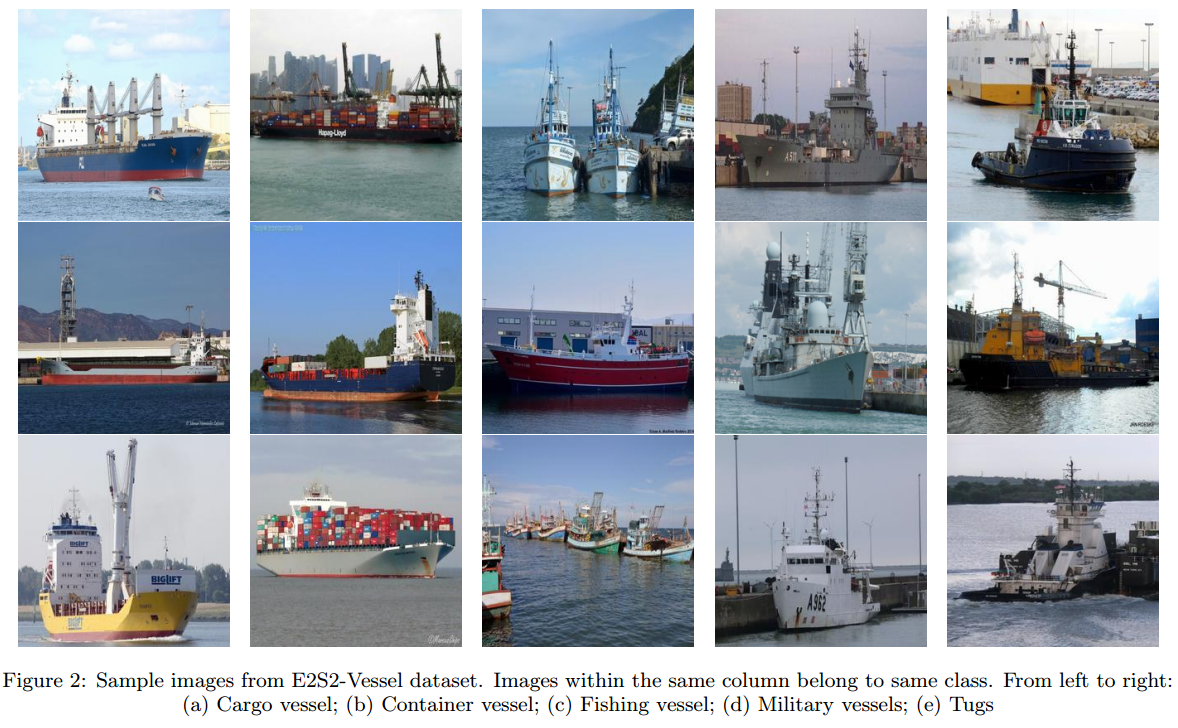
\includegraphics[width=\textwidth]{pic/figure.png}\\
        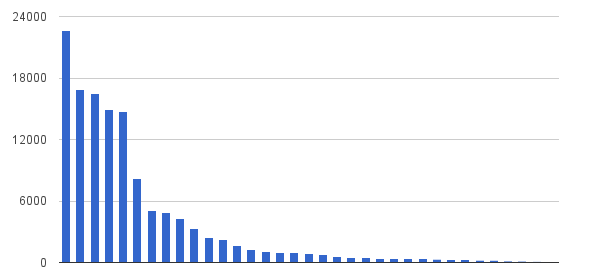
\includegraphics[width=\textwidth]{pic/image_dist.png}\\
    \end{column}
\end{columns}
\end{frame}

\begin{frame}{Dataset - Prepossessing}
\begin{itemize}
    \item After refinement: $130,000$ images in E2S2-Vessel
    \begin{itemize}
        \item Training set: $80\% - 103,000$ images
        \item Validation set: $20\% - 27,000$ images
    \end{itemize}
    \item Squashing all images to size $256\times256$
    \item Converting all images to LMDB format
    \item Shuffling the order of images in both training and validation sets
\end{itemize}
\end{frame}

\subsection{Training the CNN}
\begin{frame}{Training - Hardware}
    \begin{itemize}
        \item Commodity hardware specifications
        \begin{itemize}
            \item CPU: Intel Core 2 Quad Q9550 @2.38GHz
            \item RAM : 4GB DDR3
            \item GPU : NVIDIA Geforce GTX 560 Ti with 2GB of memory
        \end{itemize}
        \centering
        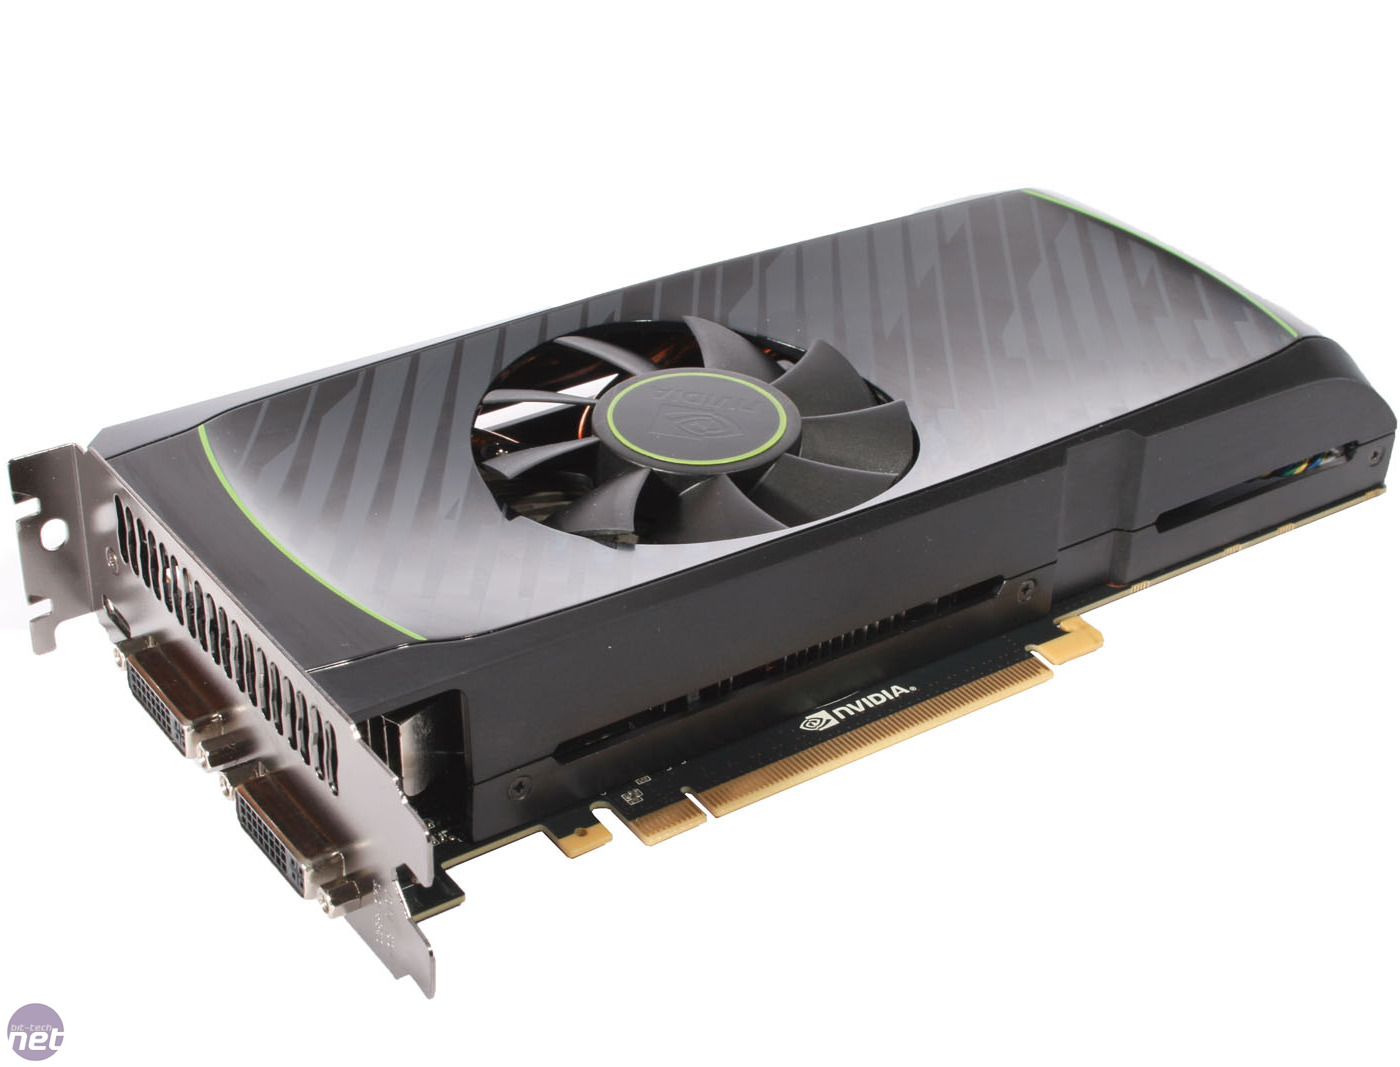
\includegraphics[width=0.5\textwidth]{pic/gtx560.jpg}
    \end{itemize}
\end{frame}

\subsection{Training the CNN}
\begin{frame}{Training - Models}
    \begin{itemize}
        \item Commodity hardware specifications
        \begin{itemize}
            \item CPU: Intel Core 2 Quad Q9550 @2.38GHz
            \item RAM : 4GB DDR3
            \item GPU : NVIDIA Geforce GTX 560 Ti with 2GB of memory
        \end{itemize}
        \centering
        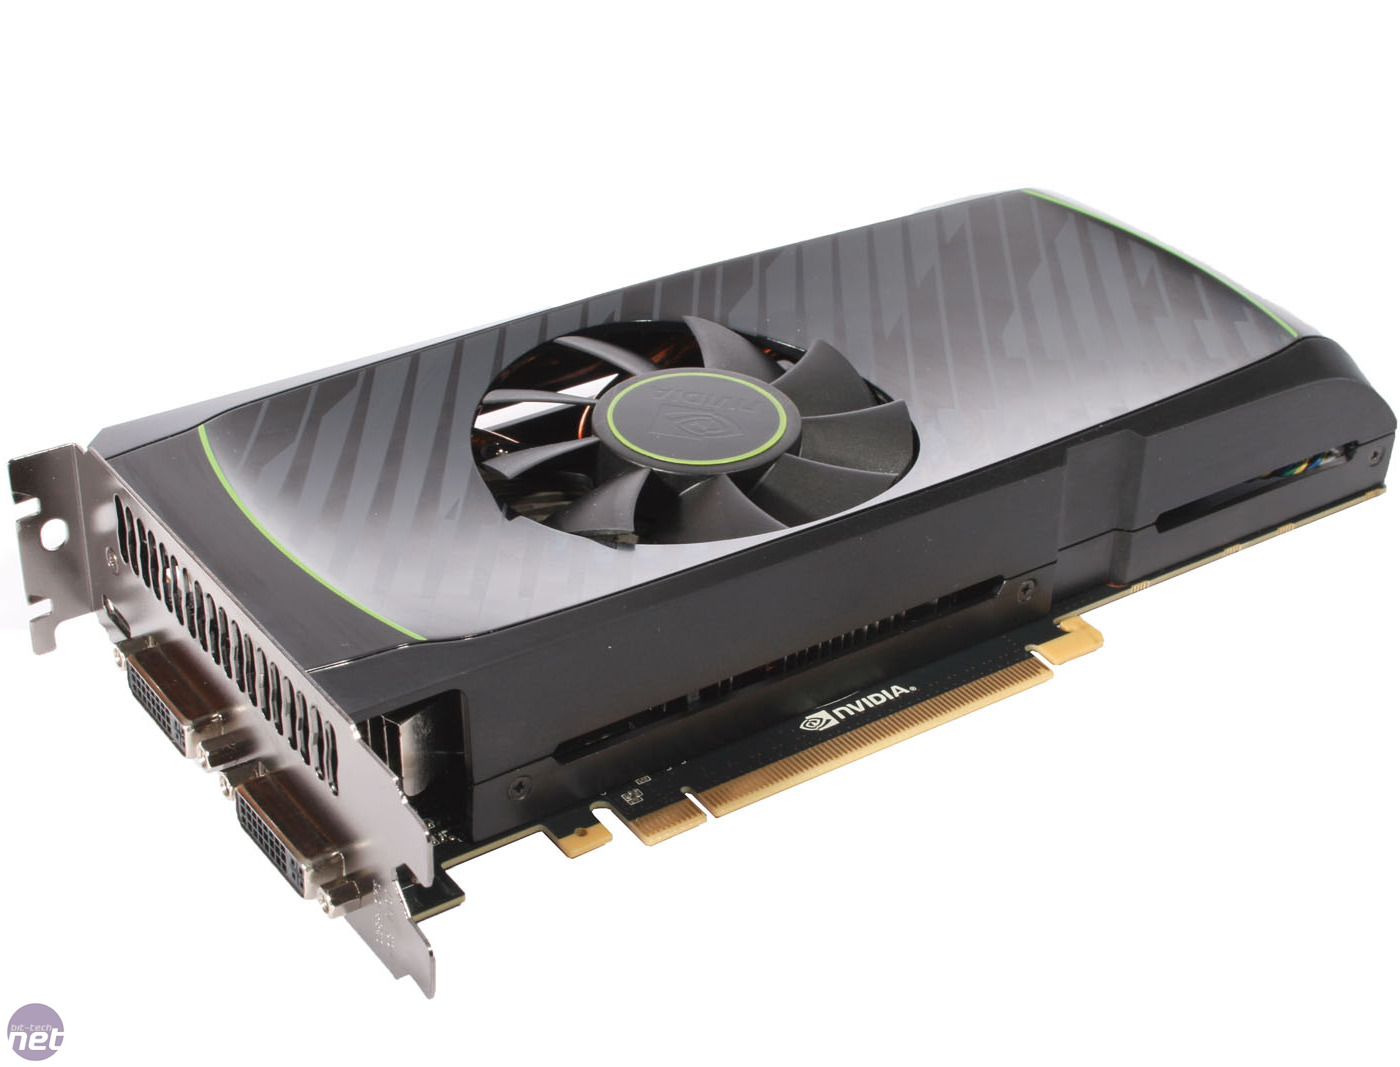
\includegraphics[width=0.5\textwidth]{pic/gtx560.jpg}
    \end{itemize}
\end{frame}

\begin{frame}{Training - Process}
    \begin{itemize}
        \item Commodity hardware specifications
        \begin{itemize}
            \item CPU: Intel Core 2 Quad Q9550 @2.38GHz
            \item RAM : 4GB DDR3
            \item GPU : NVIDIA Geforce GTX 560 Ti with 2GB of memory
        \end{itemize}
        \centering
        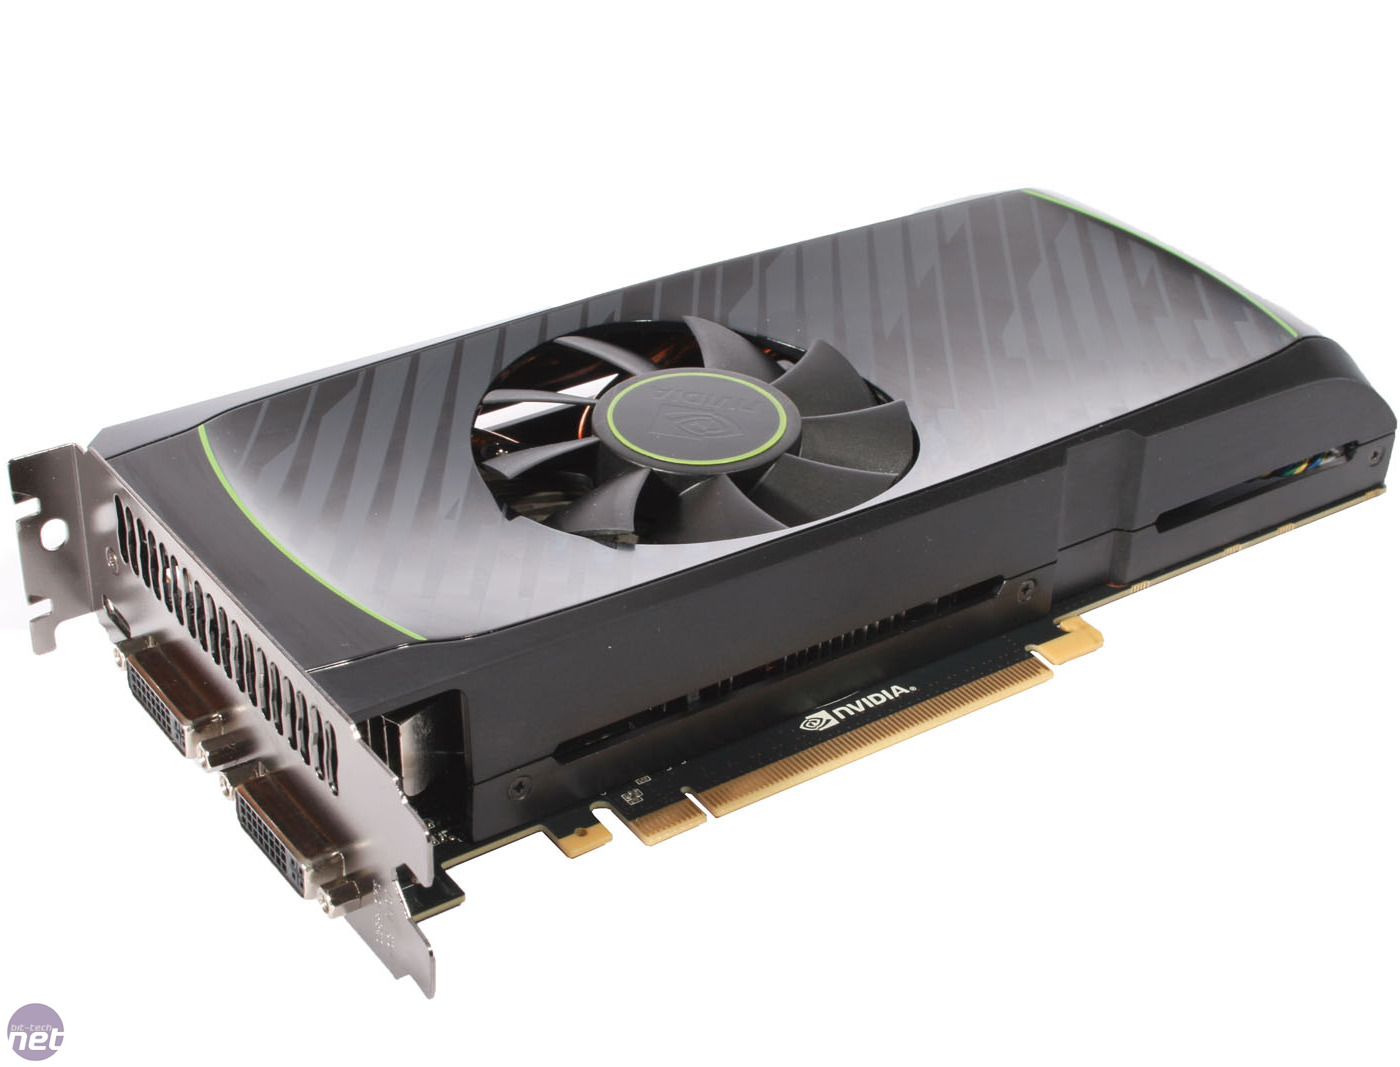
\includegraphics[width=0.5\textwidth]{pic/gtx560.jpg}
    \end{itemize}
\end{frame}

\section{Results}
\begin{frame}{Results}
\end{frame}
\end{document}



